\section{A Positive Box Removes the Veto}
\label{sec:failure}

\begin{table*}[t]
    \centering
    \small
    \begin{tabular}{@{}llr cc cccc@{}}
\toprule
 & & & \multicolumn{2}{c}{Text only} & \multicolumn{4}{c}{Text + positive box on the largest object} \\
\cmidrule(lr){4-5}\cmidrule(l){6-9}
Images & Absence & Episodes & $s_p\!\geq\!0$ & any mask & $s_p\!\geq\!0$ & $s_p\!=\!10$ & any mask & boxed object returned \\
\midrule
COCO & 80 classes & 1,500 & 1.9 & 1.3 & 99.9 {\scriptsize[99.7, 100.0]} & 59.1 & 99.9 & 89.5 {\scriptsize[86.9, 92.0]} \\
LVIS, selection & verified & 1,500 & 1.5 & 1.1 & 99.8 {\scriptsize[99.5, 100.0]} & 60.0 & 99.8 & 96.6 {\scriptsize[95.2, 97.9]} \\
LVIS, held-out & verified & 1,500 & 1.6 & 1.3 & 99.5 {\scriptsize[98.9, 99.9]} & 59.0 & 99.5 & 96.8 {\scriptsize[95.5, 98.1]} \\
\bottomrule
\end{tabular}

    \caption{\textbf{Absent phrases with and without a positive exemplar.}
    Percent of episodes.
    $\spres \geq 0$: the presence head does not reject.
    $\spres = 10$: the logit is at its upper clamp.
    \emph{Boxed object returned}: a kept mask covers the anchor (IoU $> 0.5$).
    The LVIS held-out row was run under criteria fixed after the first two rows.}
    \label{tab:veto}
\end{table*}

\begin{figure}[t]
    \centering
    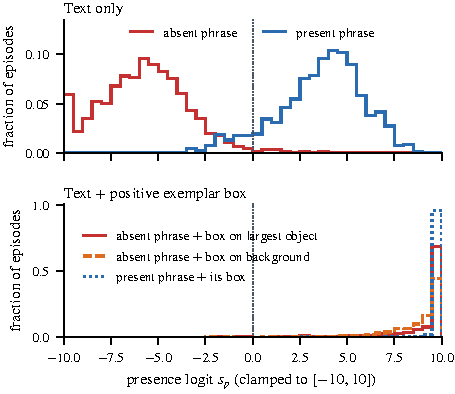
\includegraphics[width=\linewidth]{fig/presence.pdf}
    \caption{\textbf{Presence logits on the LVIS held-out images.}
    Top: text alone separates absent from present phrases.
    Bottom: with a positive box, absent phrases move to the top of the range, whether the box is on an object or on background, and overlap the consistent prompts.}
    \label{fig:presence}
\end{figure}

\paragraph{Text alone is rejected.}
Without an exemplar the presence head does what the \sam{} paper says.
On the held-out images an absent phrase has $\spres \geq 0$ in 1.6\% of 1,500 episodes and returns a mask in 1.3\% (\cref{tab:veto}).
The mean logit is $-5.69$ for absent phrases and $3.57$ for phrases of categories that are present and exhaustively annotated, and the two separate with an AUROC of 0.993 (\cref{fig:presence}, top).

\paragraph{With a box, nothing is rejected.}
Adding the anchor box as a positive exemplar to the same phrases makes $\spres \geq 0$ in 99.5\% of episodes [98.9, 99.9].
The median logit is 10, the clamp, and 59.0\% of episodes sit exactly there.
A mask is returned in 99.5\% of episodes, and in 96.8\% [95.5, 98.1] a kept mask covers the anchor.
The model returns one mask in the median episode: it segments the boxed object and reports it as the absent concept.
The selection set gives 99.8\% and 96.6\%.
On COCO, where absence is weaker, the rates are 99.9\% and 89.5\%.

\paragraph{The box overrides a competing name.}
On COCO we also named a \emph{different} category that is present in the image while boxing the anchor.
In 421 such episodes a kept mask covers the anchor in 86.5\%, and the named category's masks reach an IoU above 0.5 with their ground truth in 10.5\%.
The \sam{} paper states that prompts must be consistent or the behaviour is undefined~\cite{carion2026sam3}.
Our point is narrower: the model has a head whose job is to detect that a phrase does not match the image, and the exemplar silences it, so the inconsistency is returned with full confidence.

\paragraph{A rank metric hides the failure.}
Our first criterion for this claim failed.
Phase 1 required the present-versus-absent AUROC of $\spres$ to fall to 0.60 or below under a box; it fell from 0.996 to 0.673.
The residual ranking lives inside the positive range: consistent prompts are at the clamp in 92.4\% of episodes and absent phrases in 59.1\%.
A threshold-free metric rewards that ordering although no absent phrase is rejected at the model's operating point.
From phase 2 on, the claim is stated at the decision level, as the fraction with $\spres \geq 0$, and that is the form that passed on both LVIS sets.
